\section{WaveNet tapasztalatok}

Első célnak a beszédszintézis WaveNet alapú megoldását tűztük ki. Ennek lényege az aktuális időpillanatban a hanghullám értékénék az előző, már meghatározott értékek és a szövegfeldolgozásból kapott címkék segítségével történő meghatározása. Két rendszertervet dolgoztunk ki, azzal a különbséggel hogy a fonéma hosszának a becslése egy külön hálóban történik vagy a kimenetről van visszavezetve. Utóbbi esetben a hullámérték mellett lenne egy másik kimeneti érték is, amely azt adná meg hogy kezdődjön-e az új fonéma.

\begin{centering}
	\textbf{WaveNet külön fonéma becsült hálóval}\par\medskip\centering
	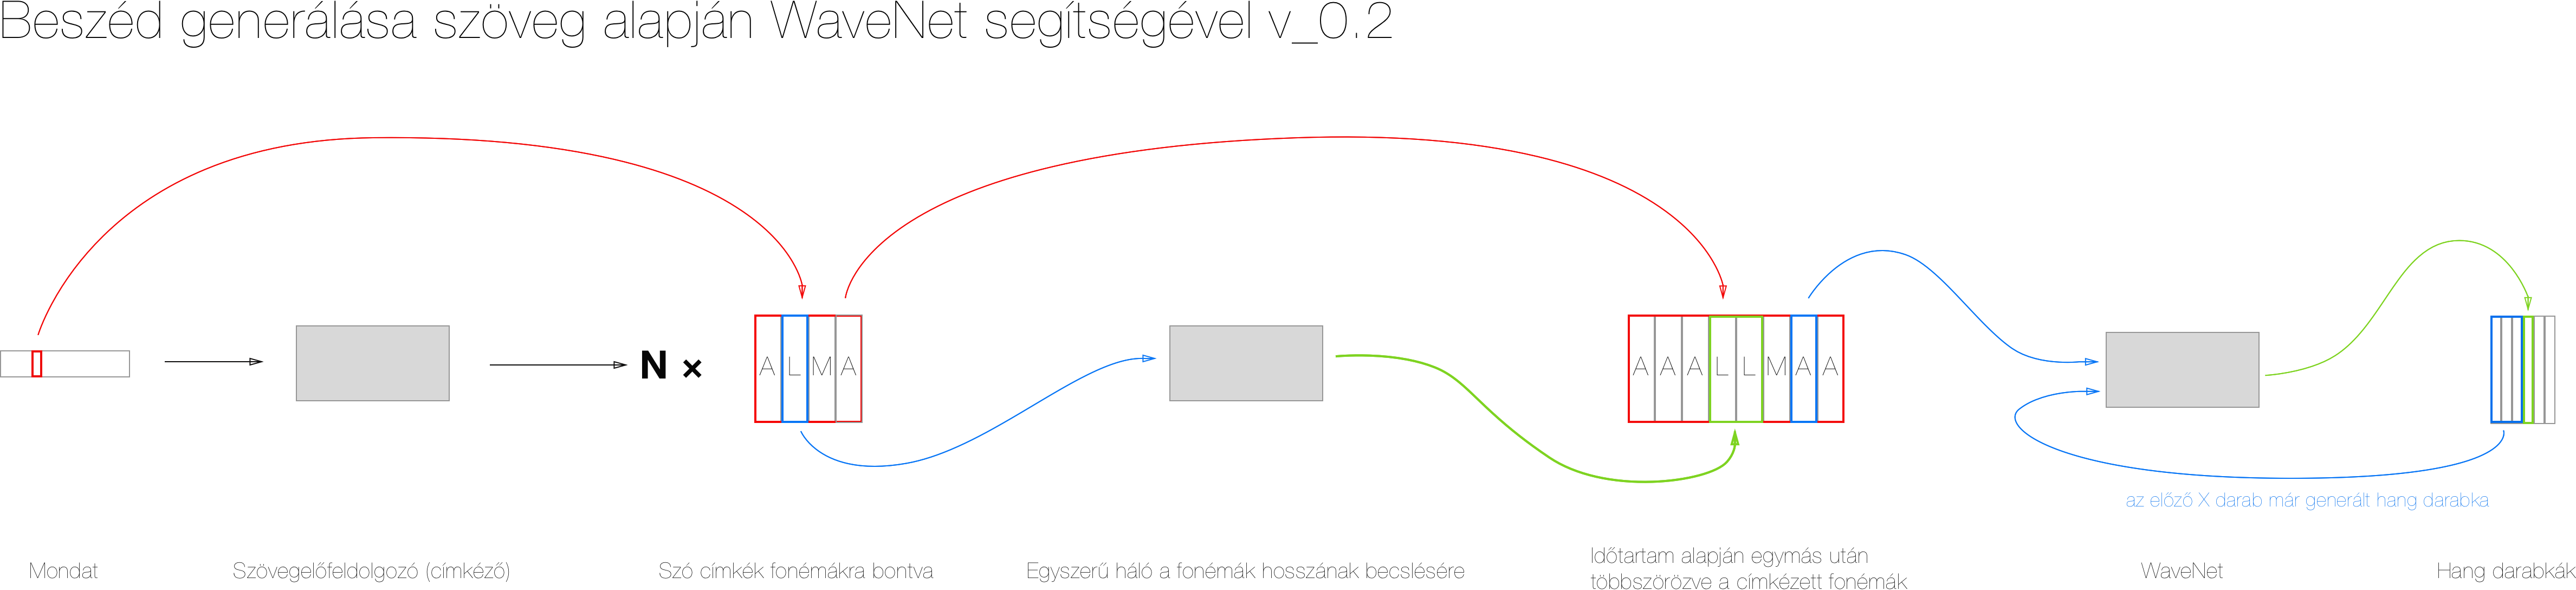
\includegraphics[width=\textwidth,keepaspectratio]{wavenet_0_2}
	
	\textbf{WaveNet fonéma becsléssel kiegészítve}\par\medskip
	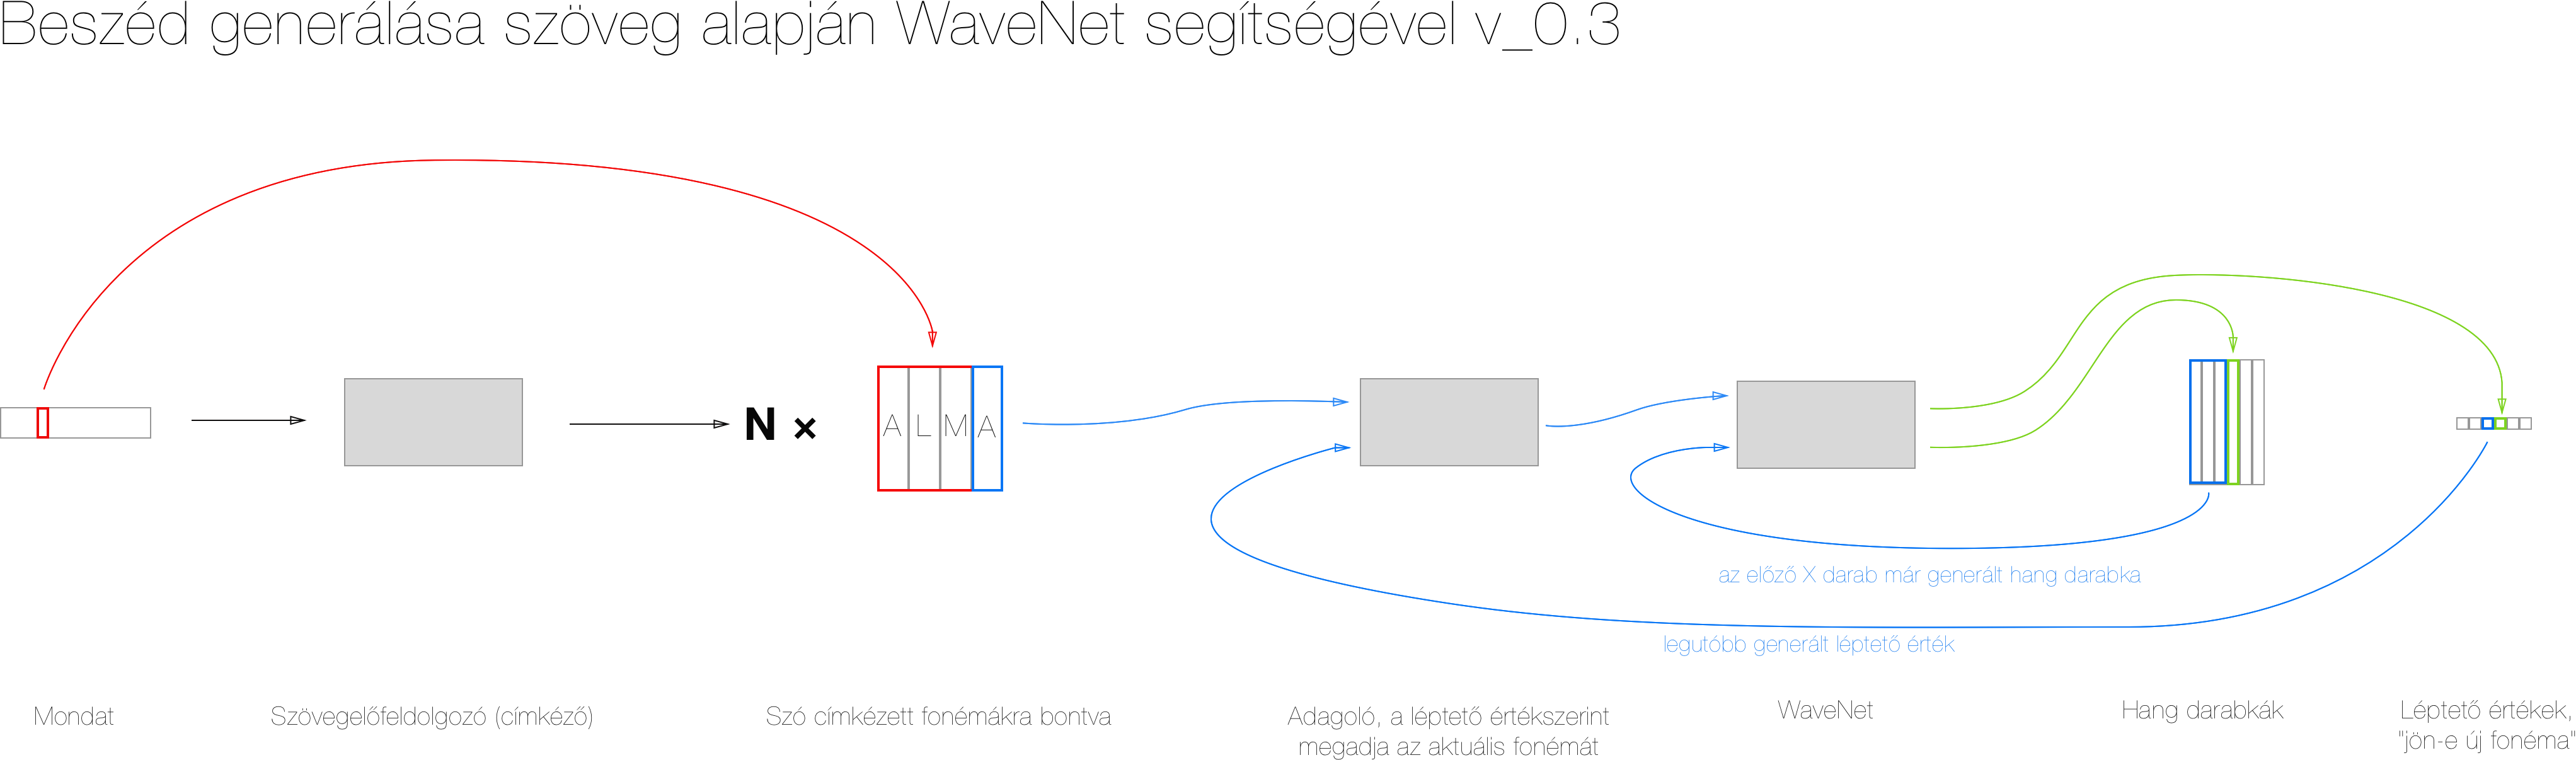
\includegraphics[width=\textwidth,keepaspectratio]{wavenet_0_3}
\end{centering}

A megvalósítás során először már meglévő, GitHub-on elérhető implementációkat próbáltunk ki. Ezek közül az egyiket sikerült egy adott mondatra tanítanunk, azt vissza tudta generálni pontosan. Azonban más mondatokkal való továbbtanítás esetén már nem volt működőképes.

Ezután saját implementációval próbálkoztunk a DeepMind által publikált cikk alapján. Ez az implementáció lényegesen egyszerűbb volt mint a cikkben meghatározott, célunk csak valamilyen kis zörej előállítása volt. Azonban konstans (néma) hangon kívül mást nem sikerült előállítanunk.

A fent említett kísérletek után egyértelművé vált, hogy túl nagy feladatba kezdtünk bele. Ezért visszaléptünk az eredeti célunktól és folytatásképpen a hagyományos DNN alapú beszédszintézissel haladtunk tovább.